\documentclass{scrartcl}
\usepackage[utf8]{inputenc}
\usepackage[german]{babel}
\usepackage{amsmath}
\usepackage{amssymb}
\usepackage{natbib}
\usepackage{graphicx}
\usepackage{subcaption}
\usepackage{float}
\floatplacement{figure}{htbp}
\floatplacement{table}{htbp}
\usepackage[
  section, % Floats innerhalb der Section halten
  below,   % unterhalb der Section aber auf der selben Seite ist ok
]{placeins}
\usepackage{subcaption}
\usepackage{xfrac}
\usepackage{enumitem}

\begin{document}

\section*{Übungsblatt 2 -- Cerberus}

    \subsection*{Aufgabe 1}

        Im Folgenden soll das $512 \times 512$ Bild aus Abbildung \ref{fig:bild} mithilfe der Singulärwertzerlegung
        \begin{equation*}
            \mathbf{A} = \mathbf{U} \cdot \mathbf{\Sigma} \cdot \mathbf{V}^{\text{T}}
        \end{equation*}
        und der Rang-\textit{k}-Approximation komprimiert werden.
        %\begin{figure}
        %    \centering
        %    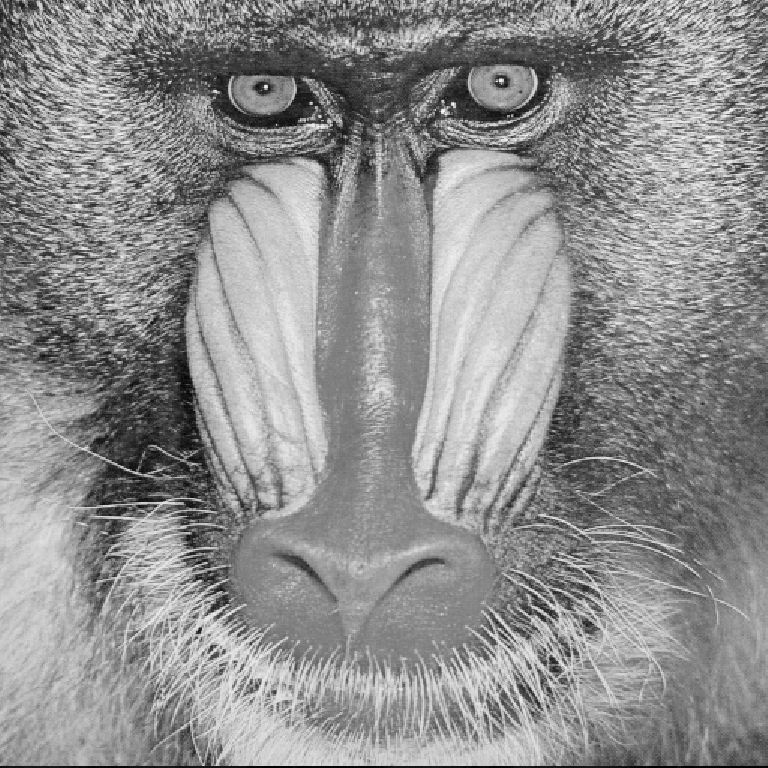
\includegraphics[width=0.5\textwidth]{A1/build/bild.pdf}
        %    \caption{Originalbild.}
        %    \label{fig:bild}
        %\end{figure}
        Die Rekonstruktion und Approximation erfolgt mithilfe von 
        \begin{equation*}
            \mathbf{\tilde{A}} = \sum_{i = 1}^{k} \sigma_i \vec{u}_i \vec{v}_i^{\text{T}} \:\:\: \text{mit} \: k \leq 512.
        \end{equation*}
        \begin{center}
            \tiny{$\sigma_i \: \hat{=}$ i-tes Diagonalelement von $\mathbf{\Sigma}$, $\vec{u}_i \: \hat{=}$ i-ter Spaltenvektor von $\mathbf{U}$,
                  $\vec{v}_i \: \hat{=}$ i-iter Spaltenvektor von $\mathbf{V}$.}
        \end{center}
        Die approximierten Bilder für $k = 10, 20, 50$ befinden sich in Abbildung \ref{fig:approx}.
        \begin{figure}
            \centering
            \begin{subfigure}[b]{0.3\textwidth}
                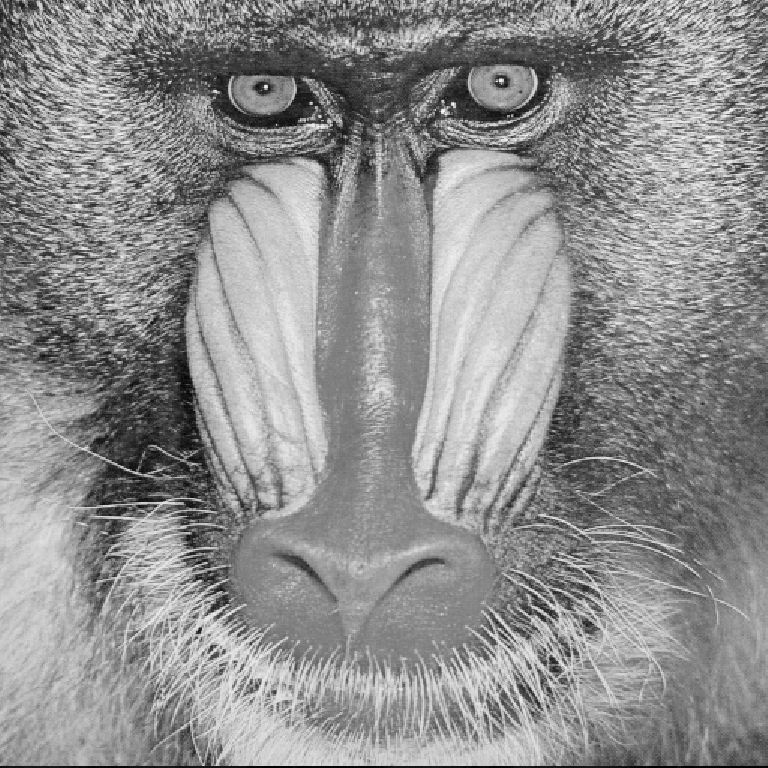
\includegraphics[width=\textwidth]{A1/build/bild.pdf}
                \caption{Originalbild.}
                \label{fig:bild}
            \end{subfigure}
            ~ %add desired spacing between images, e. g. ~, \quad, \qquad, \hfill etc. 
            %(or a blank line to force the subfigure onto a new line)
            \begin{subfigure}[b]{0.3\textwidth}
                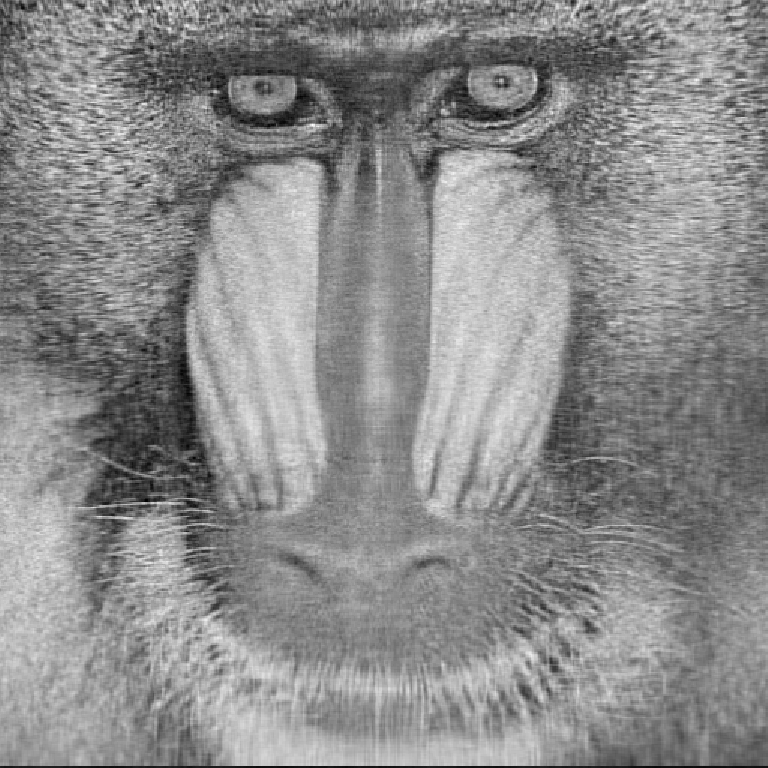
\includegraphics[width=\textwidth]{A1/build/A50.pdf}
                \caption{$k=50$.}
                \label{fig:A50}
            \end{subfigure}
            
             %add desired spacing between images, e. g. ~, \quad, \qquad, \hfill etc. 
              %(or a blank line to force the subfigure onto a new line)
            \begin{subfigure}[b]{0.3\textwidth}
                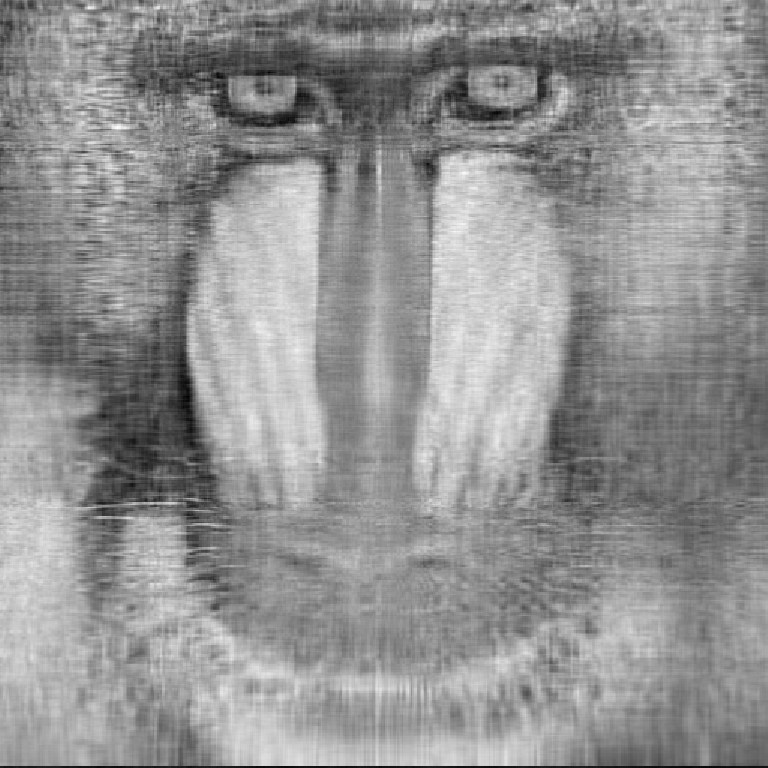
\includegraphics[width=\textwidth]{A1/build/A20.pdf}
                \caption{$k=20$.}
                \label{fig:A20}
            \end{subfigure}
            ~
            \begin{subfigure}[b]{0.3\textwidth}
                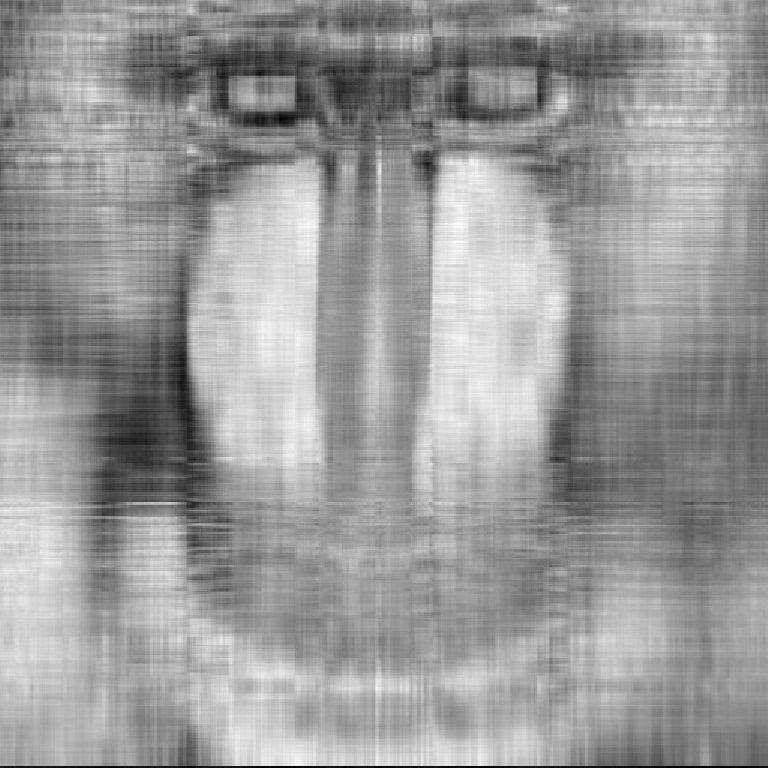
\includegraphics[width=\textwidth]{A1/build/A10.pdf}
                \caption{$k=10$.}
                \label{fig:A10}
            \end{subfigure}
            \caption{Approximation von Abbildung \ref{fig:bild} für verschiedene $k$.}\label{fig:approx}
        \end{figure}
        Die SVD scheint sich gut zur Kompression zu eignen, da sich das Bild, wie in Abbildung \ref{fig:A50} zu sehen, mit nur knapp
        $10 \, \%$ der Singulärwerte schon sehr gut rekonstruieren lässt. Selbst bei einer so extremen Kompression wie in Abbildung
        \ref{fig:A10} ist das Motiv noch ganz grob zu erkennen.
	
    \subsection*{Aufgabe 2}
    
		Ein Profiler wird verwendet um die Geschwindigkeit verschiedener Abschnitte einer LU-Zerlegung zu überprüfen.
		Ein Timer überprüft die benötigte Zeit
		\begin{enumerate}
		\item eine $N\times N$-Matrix $M$ und einen $N$d-Vektor $b$ mit zufälligen Einträgen zu erzeugen
		\item eine LU-Zerlegung durchzuführen
		\item das Problem $Mx = b$ zu lösen
		\end{enumerate}				
		Die Zeit $t$, die für die einzelnen Schritte benötigt wird, wird in Abhängigkeit von der Matrixgröße $N$ doppelt-logarithmisch aufgetragen. Die LU-Zerlegung mithilfe der \texttt{eigen}-Library unterstützt Multithreading und kann somit abhängig vom verwendeten Prozessor beschleunigt werden (in diesem Fall bis zu $15\%$). Generell zeigt sich, dass die benötigte Zeit von der verwendeten CPU abhängt, jedoch lässt sich sowohl bei logarithmisch (\ref{fig:time}) wie auch linear (\ref{fig:time_lin}) ansteigender Matrizengröße $N$ ein Trend erkennen.\\ Bei großen Problemen ($N\gtrsim 200$) lässt sich die benötigte Zeit für jeden der drei Teilschritte in Abb.\ref{fig:fit} als $\mathcal{O}(N^3)$ extrapolieren.
 		\begin{figure}[h!]
 		\centering
 		\begin{subfigure}{0.3\textwidth}
		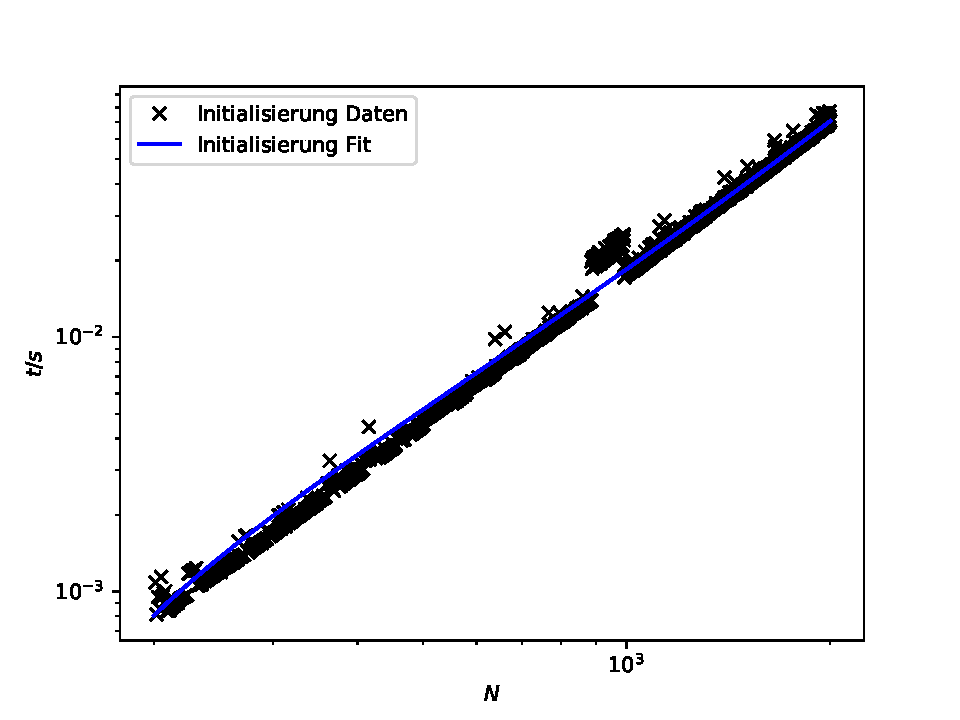
\includegraphics[width=\textwidth]{A2/build/t1_200.pdf}
		\end{subfigure}
		\begin{subfigure}{0.3\textwidth}
		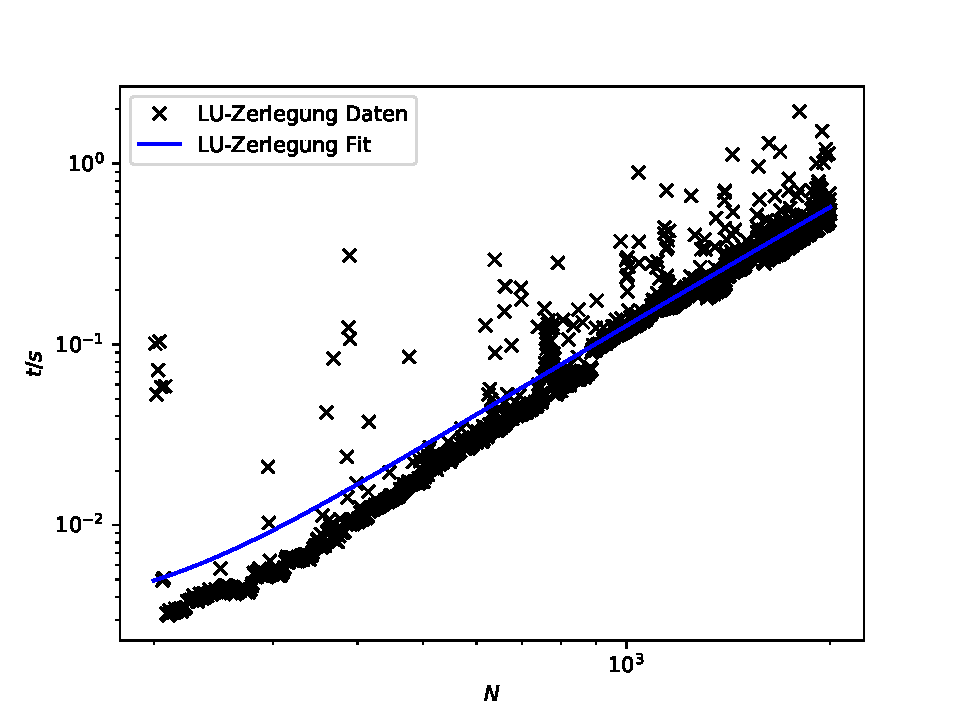
\includegraphics[width=\textwidth]{A2/build/t2_200.pdf}
		\end{subfigure}
		\begin{subfigure}{0.3\textwidth}
		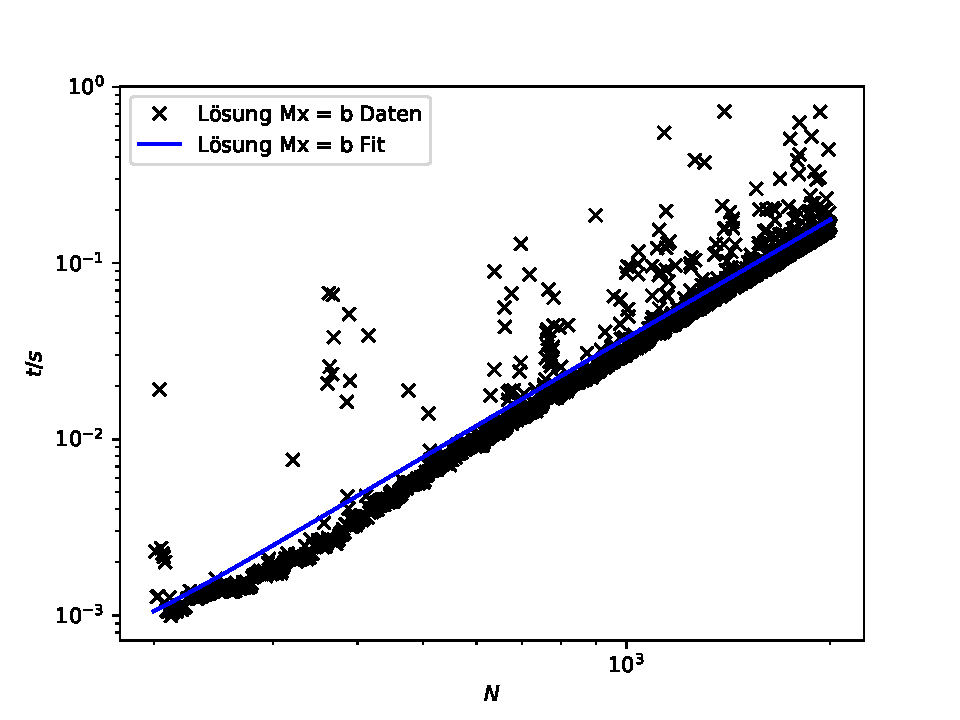
\includegraphics[width=\textwidth]{A2/build/t3_200.pdf}
		\end{subfigure}
		\caption{Die Daten der drei verschiedenen Teilschritte gefittet an ein Polynom 3. Grades für große $N$}
		\label{fig:fit}
 		\end{figure}
		\begin{figure}[h!]
		\centering
		\begin{subfigure}{0.8\textwidth}
		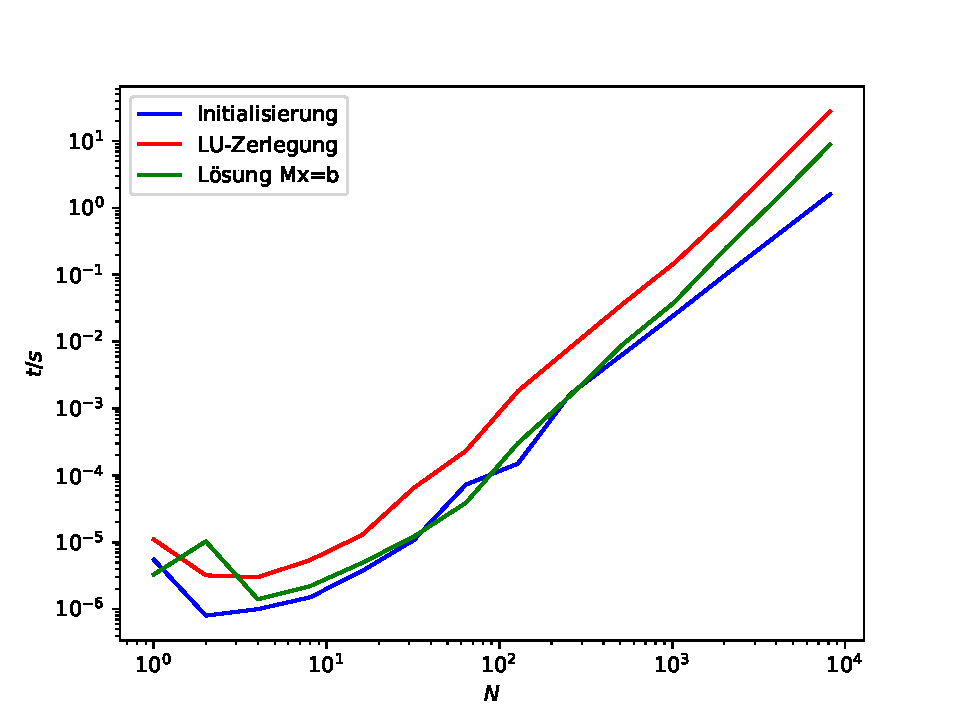
\includegraphics[width=\textwidth]{A2/build/timers.pdf}
		\end{subfigure}
		\begin{subfigure}{0.4\textwidth}
		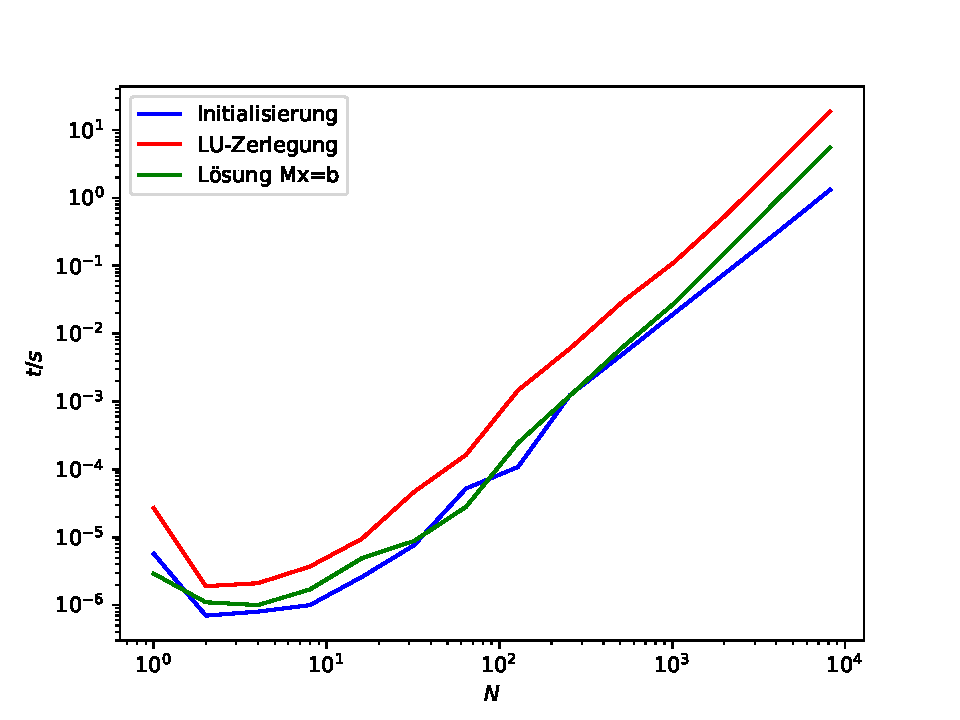
\includegraphics[width=\textwidth]{A2/Dann_halt_so/timers_PC.pdf}
		\end{subfigure}
		\begin{subfigure}{0.4\textwidth}
		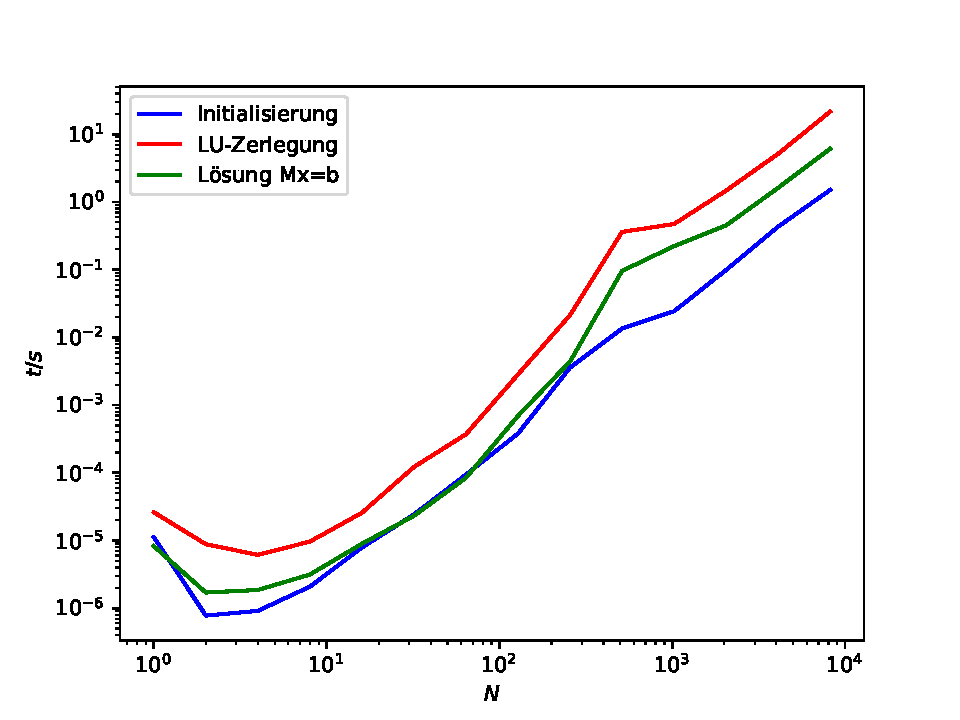
\includegraphics[width=\textwidth]{A2/Dann_halt_so/timers_Prd.pdf}
		\end{subfigure}
		\caption{Die benötigte Zeit für Operationen bei logarithmisch ansteigendem $N$ mit verschiedenen CPUs.}
		\label{fig:time}
		\end{figure}
		\begin{figure}[h!]
		\centering
		\begin{subfigure}{0.8\textwidth}
		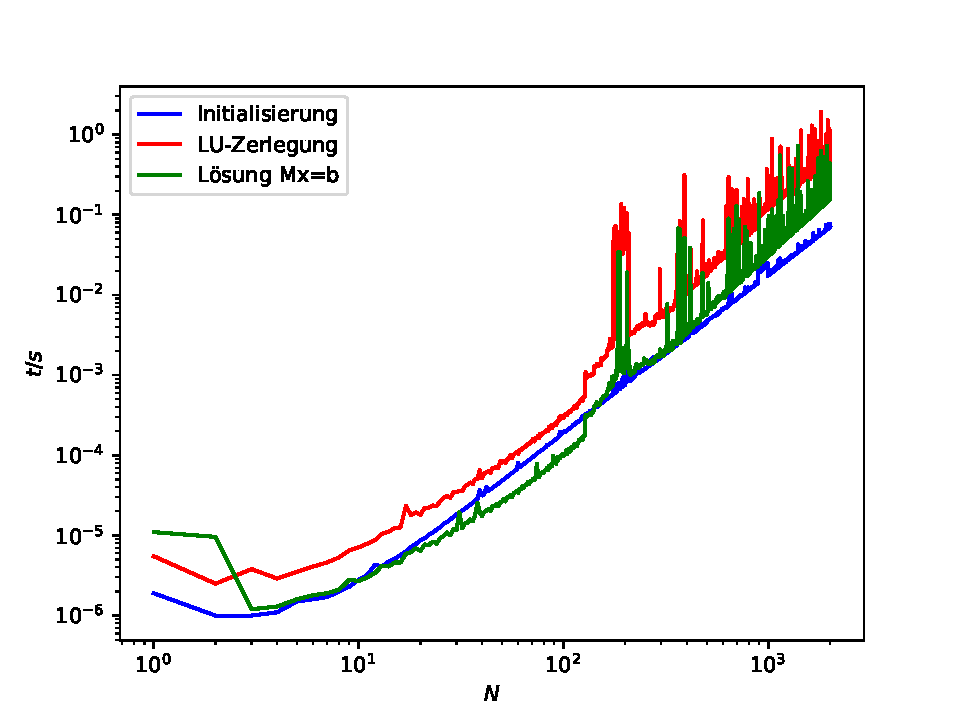
\includegraphics[width=\textwidth]{A2/build/timers_lin.pdf}
		\end{subfigure}
		\begin{subfigure}{0.4\textwidth}
		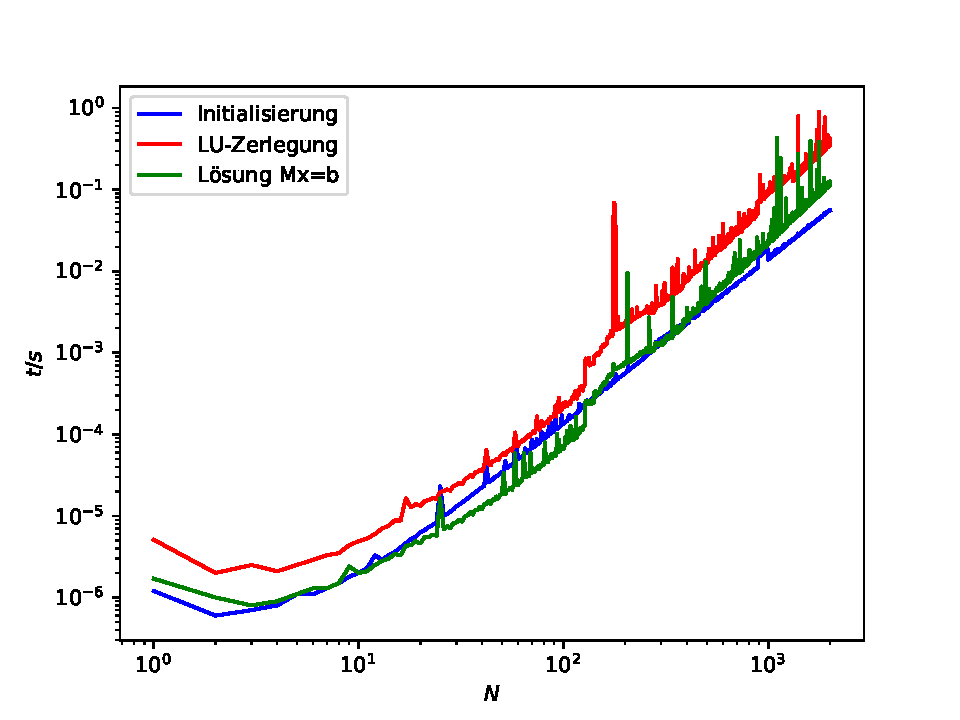
\includegraphics[width=\textwidth]{A2/Dann_halt_so/timers_lin_PC.pdf}
		\end{subfigure}
		\begin{subfigure}{0.4\textwidth}
		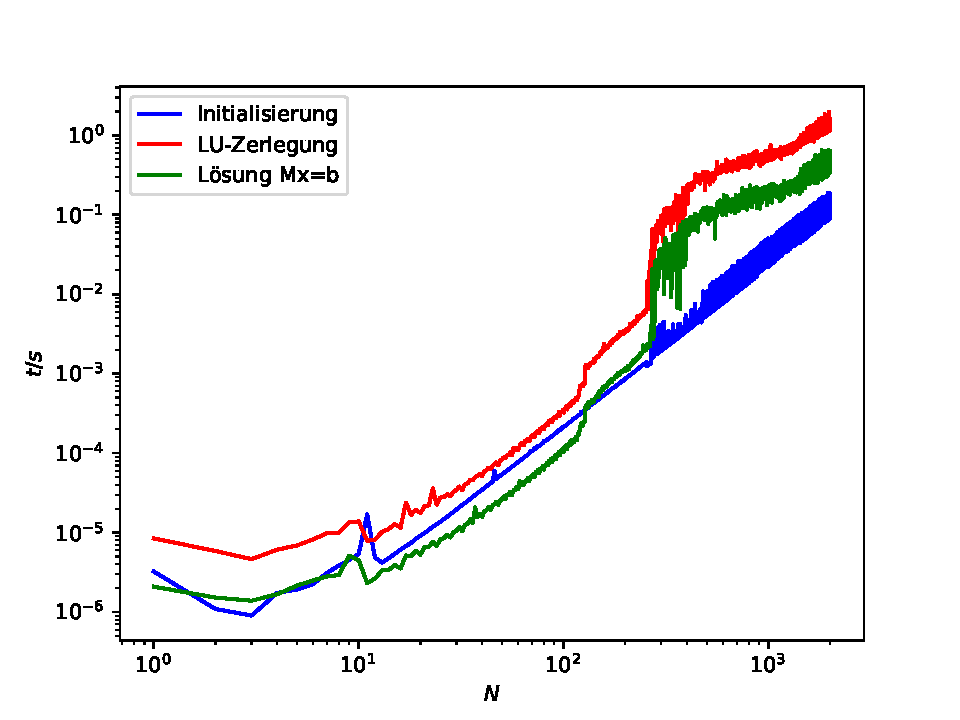
\includegraphics[width=\textwidth]{A2/Dann_halt_so/timers_lin_Prd.pdf}
		\end{subfigure}
		\caption{Die benötigte Zeit für Operationen bei linear ansteigendem $N$ mit verschiedenen CPUs.}
		\label{fig:time_lin}
        \end{figure}

        \FloatBarrier
        \subsection*{Aufgabe 3}
        In dieser Aufgabe wurde ein Profiler genutzt, um die Laufzeiten verschiedener Algorithmen zum Lösen eines linearen Gleichungssystems der Form 
        \begin{equation}
            Mx=b
        \end{equation}
        \begin{center}
            \tiny{($M \hat{=} \text{Zufällige N x N Matrix}$, $x, b \hat{=} \text{Vektor mit Dimension N}$)}
        \end{center}
        zu bestimmen. Dabei wird $N$ für alle Methoden linear in dem Intervall $[1, 1000]$ variiert. 
        Die Laufzeiten werden für die folgenden Methoden verglichen: 
        \begin{enumerate}
            \item Multiplikation von $M^{-1}$ auf der linken Seite \label{M1}
            \item Partielle LU-Zerlegung
            \item Vollständige LU-Zerlegung.
        \end{enumerate} 
        Wie in Abbildung \ref{fig:A3times} zu sehen ist, wird für die partielle LU-Zerlegung am wenigsten Zeit benötigt. Es sei zusätzlich erwähnt, dass die partielle LU-Zerlegung zusätzlich vom Multithreading profitiert \footnote[1]{https://eigen.tuxfamily.org/dox/TopicMultiThreading.html}, was ebenfalls Laufzeit sparen kann.

        \begin{figure}[H]
            \centering
            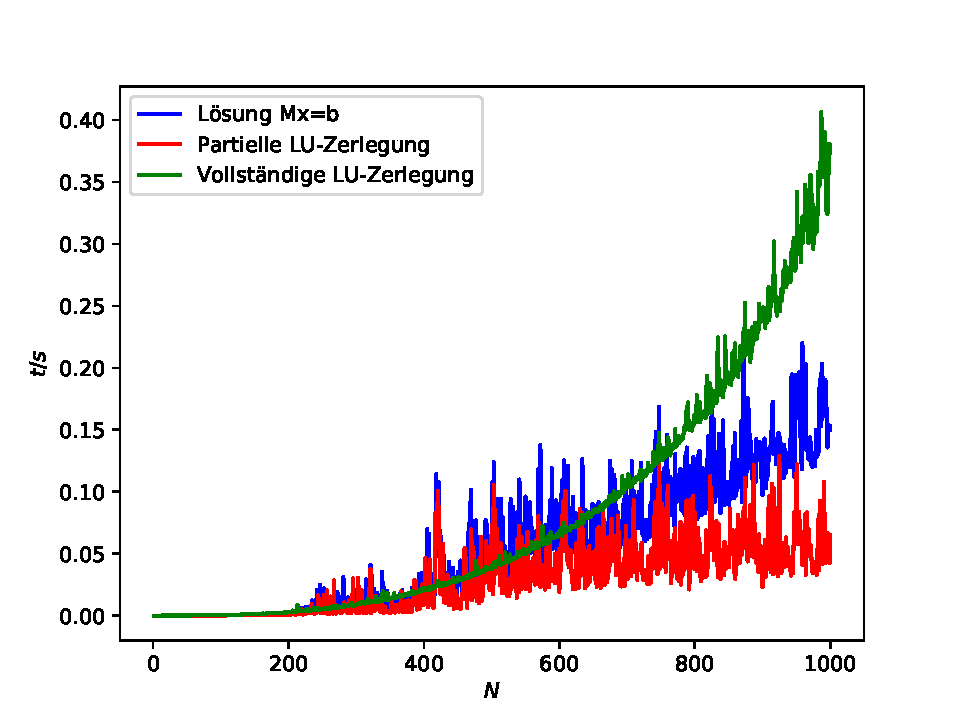
\includegraphics[scale=0.7]{A3/build/timers.pdf}
            \caption{Laufzeit der verschiedenen Methoden.}
            \label{fig:A3times}
        \end{figure}

        Anschließend wurde verglichen, ob auch alle Algorithmen das gleiche Ergebnis liefern. Als Maß dafür wurde hier die "squared Euclidean distance" gewählt, die die zwischen der partiellen (vollstädnigen) LU-Zerlegung und der Methode \ref{M1} berechnet wurde. Wie in in Abbildung \label{fig:A3devs} zu sehen ist, sind die Abstände für die partielle LU-Zerlegung für nahezu alle $N$ kleiner.

        \begin{figure}[H]
            \centering
            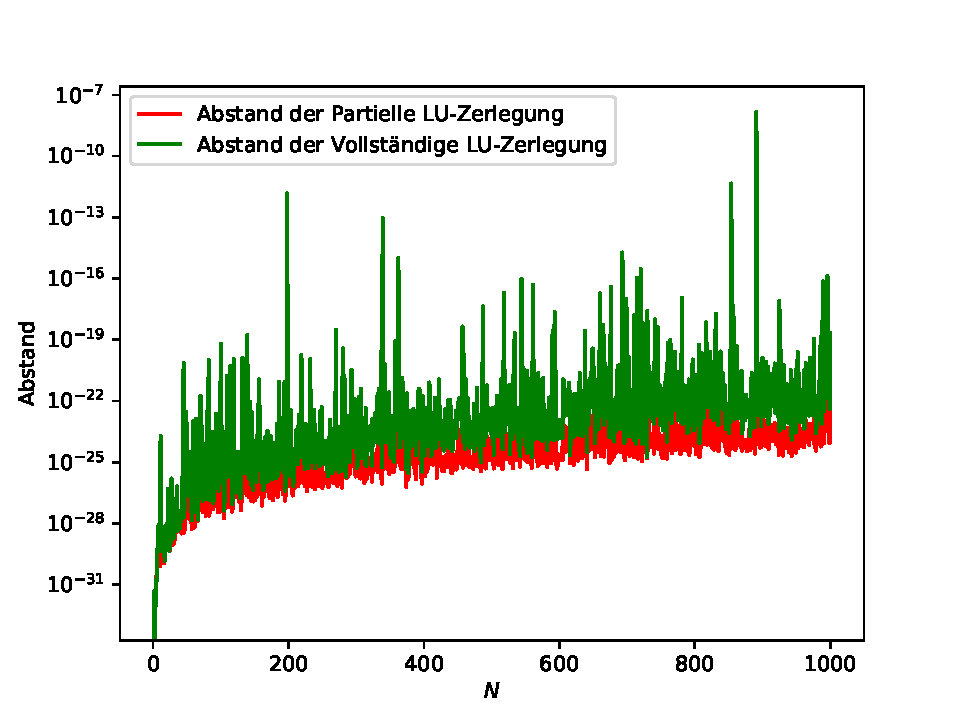
\includegraphics[scale=0.7]{A3/build/devs.pdf}
            \caption{Abweichung der Partiellen und vollständigen LU-Zerlegung zu Methode \ref{M1}.}
            \label{fig:A3devs}
        \end{figure}

        Insgesamt ist also die partielle LU-Zerlegung zu bevorzugen, da die Laufzeit  – bis auf wenige Ausnahmen  – für alle N im untersuchten Intervall am geringsten ist. Ebenso scheinen die Ergebnisse genauer als die der vollständigen LU-Zerlegung zu sein.

\end{document}
